\chapter{Neutrino physics} %%%%%%%%%%%%%%%%%%%%%%%%%%%%%%%%%%%%%%%%%%%%%%%%%%%%%%%%%%%%%%%%%%%%%%%
\label{chap:theory} %%%%%%%%%%%%%%%%%%%%%%%%%%%%%%%%%%%%%%%%%%%%%%%%%%%%%%%%%%%%%%%%%%%%%%%%%%%%%%

Vast numbers of neutrinos pass through everything around us each second, all incredibly unlikely
to interact even once. Nearly a century since they were first proposed, neutrinos have now
conclusively been proven to undergo oscillations between their flavour states. This discovery has
opened the door to physics beyond that initially conceived within the Standard Model, which may
reveal new, fundamental insights into the universe. This chapter aims to outline the historical
context, theoretical background and open questions surrounding the neutrino.

\section{A history} %%%%%%%%%%%%%%%%%%%%%%%%%%%%%%%%%%%%%%%%%%%%%%%%%%%%%%%%%%%%%%%%%%%%%%%%%%%%%%
\label{sec:theory_history} %%%%%%%%%%%%%%%%%%%%%%%%%%%%%%%%%%%%%%%%%%%%%%%%%%%%%%%%%%%%%%%%%%%%%%%

\subsection{Discovery of the neutrinos} %%%%%%%%%%%%%%%%%%%%%%%%%%%%%%%%%%%%%%%%%%%%%%%%%%%%%%%%%%
\label{sec:theory_history_neutrinos} %%%%%%%%%%%%%%%%%%%%%%%%%%%%%%%%%%%%%%%%%%%%%%%%%%%%%%%%%%%%%

In the early 20th century, beta decays were assumed to follow the simple two-body process,
$A\rightarrow B + e$, where $A$ spontaneously emits a single electron. To conserve both energy and
angular momentum, the ejected electron was believed to have discrete kinetic energy, defined by
the difference in binding energies between $A$ and $B$. However, in 1914, J. Chadwick instead
measured a continuous electron energy spectrum~\cite{chadwick1914}, placing this assumption in
doubt.

W. Pauli proposed a `desperate solution' to this paradox in 1930~\cite{pauli1930}. If a light,
neutrally charged, spin $1/2$ particle was also produced in the interaction, the continuous energy
distribution could be explained. Initially, this mysterious new particle was named the
\emph{neutron}. However, to avoid confusion with the heavy baryon of the same name discovered in
1932, E. Fermi renamed it the \emph{neutrino} when he formalised beta decay in
1934~\cite{fermi1934}.

Shortly after, H. Bethe and R. Peierls~\cite{bethe1934} used Fermi's work to estimate the
cross-section for the inverse beta decay process:
\begin{equation} % INVERSE BETA DECAY EQUATION %
    \bar{\nu} + p^{+} \rightarrow n + e^{+}.
    \label{eq:inverse_beta_decay}
\end{equation}
An upper limit of $10^{-44} \mathrm{cm}^2$ was calculated, an incredibly small value, leading them
to declare `there is no practically possible way of observing the neutrino.' This statement hinted
at the vast difficulties experimentalists would face hunting down and measuring the neutrino in
the years to come.

After an initial tentative identification if 1953, F. Reines and C. Cowan made the first confirmed
observation of the neutrino in 1956~\cite{cowan1956}. Electron antineutrinos produced within the
Savannah River Plant nuclear reactor were detected via the inverse beta decay process outlined in
Eq.~\ref{eq:inverse_beta_decay}. In an underground room of the reactor building, A `club-sandwich'
detector was constructed containing three \unit{1500}{\litre} liquid scintillator tanks
interspersed with two \unit{200}{\litre} cadmium doped water target tanks. A total of 330
photomultiplier tubes measured the two characteristic signals for the interaction, allowing for
rejection of the sizeable cosmic ray background. Firstly, a prompt positron annihilation, followed
shortly afterwards by a gamma-ray burst from the neutron capture on cadmium.

A second distinct neutrino, the muon neutrino was discovered in 1962 at the Brookhaven based
Alternating Gradient Synchrotron (AGS)~\cite{danby1962}. Protons from the AGS beam incident upon a
fixed target produced charged pions which then decayed into a beam of muons and neutrinos. After
passing through steel and lead absorbers to remove the muons, neutrino interactions were detected
in a series of spark chambers.

If only a single neutrino existed, both interactions
\begin{equation} % BROOKHAVEN DECAY EQUATIONS %
    \nu+p^{+}\rightarrow\mu^{+}+n \\
    \nu+p^{+}\rightarrow e^{+}+n
\end{equation}
were expected to occur at the same rate. However, only muons, identified by a single long track in
the spark chambers were detected, confirming the existence of the muon neutrino. Not only was this
experiment the first to construct and use an artificial neutrino beam, but it also won the 1988
Nobel prize in physics.

The $Z^{0}$ and $W^{\pm}$ bosons were discovered at the CERN based Super Proton Synchrotron in
1983~\cite{arnison1983_z,arnison1983_w}. Crucially, as $Z^{0}$ bosons were expected to decay to
neutrinos, measurements made to the decay width could strongly constrain the number of neutrino
flavours. The ALEPH, DELPHI, L3 and OPAL experiments at the LEP $e^{+}e^{-}$ collider in the 1990s
made such precise measurements, indicating that the number of light active neutrino flavours to be
$2.984\pm0.008$~\cite{electroweak2006}, see Fig.~\ref{fig:z_resonance}.

\begin{figure} % Z-RESONANCE DIAGRAM %
    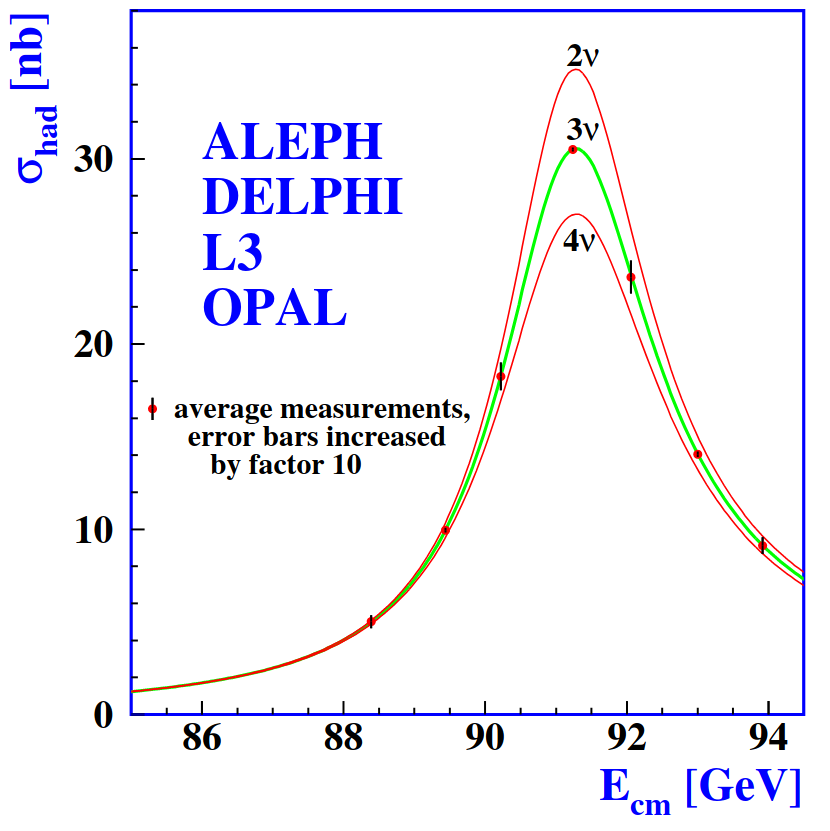
\includegraphics[origin=c,width=0.5\textwidth]{diagrams/3-theory/z_resonance.png}
    \caption[Hadron production cross-section measurements from LEP]
    {Combined hadron production cross-section measurements around the $Z^{0}$ resonance made by
        experiments at LEP. The curves show the predicted cross-section for two, three, and four
        neutrinos. Note how the data fits the three neutrino hypothesis incredibly well. Figure
        taken from Ref.\cite{electroweak2006}.}
    \label{fig:z_resonance}
\end{figure}

Combined with the discovery of the charged tau lepton in 1975~\cite{perl1975}, a third tau
neutrino was thought likely. The DONUT experiment at Fermilab finally discovered this particle in
2001~\cite{Kodama2001} using \unit{800}{\GeV} protons from the Tevatron, completing the trio of
neutrinos we know today. Any additional neutrinos must either be sterile (do not couple to the
weak force) or have a mass greater than 0.5 $m_{Z}$.

\subsection{Discovery of neutrino oscillations} %%%%%%%%%%%%%%%%%%%%%%%%%%%%%%%%%%%%%%%%%%%%%%%%%%
\label{sec:theory_history_osc} %%%%%%%%%%%%%%%%%%%%%%%%%%%%%%%%%%%%%%%%%%%%%%%%%%%%%%%%%%%%%

At the Homestake mine\footnote{The Homestake mine will also be used for the future DUNE experiment
    discussed later} in the 1960s, a large tank, placed \unit{1.5}{\mathrm{km}} underground, was
filled with \unit{400000}{\litre} of the dry cleaning fluid, perchloroethylene
($C_{4}Cl_{8}$). Its goal was to measure the solar electron neutrino flux incident upon the
earth via the interaction
\begin{equation} % HOMESTAKE CHLORINE EQUATION %
    {}^{37}Cl+\nu_{e}\rightarrow{}^{37}Ar+e^{-}.
\end{equation} %
This process allowed the neutrino flux to convert the chlorine contained within the tank into the
noble gas argon. Every few weeks the tank was purged with gaseous helium and the amount of argon
generated, and indirectly the solar neutrino flux measured.

After analysis, the number of electron neutrino interactions per ${}^{37}Cl$, per second was found
to be no greater than 3~\cite{davis1968}. When compared to the predictions made by the Standard
Solar Model ranging between 4.4 and 22~\cite{bahcall1968}, a deficit was observed. Dubbed the
\emph{solar neutrino problem}, this was initially believed to be due to an unexplained
experimental flaw. However, other experiments, such as the water Cherenkov Kamiokande
II~\cite{hirata1989} and both the SAGE and GALLEX galium based capture tanks also observed this
discrepancy~\cite{abazov1991,anselmann1994}.

A neutrino deficit was also observed indirectly in the atmospheric sector, named the
\emph{atmospheric neutrino anomaly}. Neutrinos generated from cosmic rays in the atmosphere formed
a key background to both the Kamiokande and IMD experiments, designed to primarily measure proton
decay. When evaluating the background, a deficit in the number of muon neutrinos compared to
electron neutrinos was observed~\cite{hirata1988, becker1992}. The successor to the Kamiokande
experiment Super-Kamiokande also measured a similar deficit~\cite{kajita1999}.

The phenomenon of neutrino oscillations was put forward as a solution to this problem. If
neutrinos could change flavour as they propagated, the measured deficits could be explained. The
SNO experiment finally confirmed this in 2001~\cite{ahmad2002}.

The SNO experiment consisted of a \unit{1}{\mathrm{kton}} tank of deuterium (heavy water),
equipped with 9500 photomultiplier tubes. Light from three seperate neutrino interaction channels:
\begin{align} % SNO INTERACTIONS EQUATIONS %
    \nu_{i}+e^{-} & \rightarrow \nu_{i}+e^{-} \\
    \nu_{i}+d     & \rightarrow p+n+\nu_{i}   \\
    \nu_{e}+d     & \rightarrow p+p+e^{-}
\end{align}
was measured, where $d$ is the deuterium nucleus. The first and second channels were sensitive to
all three neutrino flavours, but importantly only electron neutrinos could interact via the third
channel. By comparing the rates between the channels, SNO was able to prove to 5.3$\sigma$ that
electron neutrinos had oscillated to other flavours, whilst the total solar neutrino flux remained
constant.

\section{The Standard Model and neutrinos} %%%%%%%%%%%%%%%%%%%%%%%%%%%%%%%%%%%%%%%%%%%%%%%%%%%%%%%
\label{sec:theory_sm} %%%%%%%%%%%%%%%%%%%%%%%%%%%%%%%%%%%%%%%%%%%%%%%%%%%%%%%%%%%%%%%%%%%%%%%%%%%%

The Standard Model of particle physics describes the seventeen known fundamental subatomic
particles and their interactions. Combining both quantum chromodynamics (describing the strong
force) and electroweak theory (describing the electromagnetic and weak forces), it is a gauge
theory obeying the local gauge symmetries of $U(1) \times SU(2) \times SU(3)$. The particles,
along with their various properties, are outlined in Fig.~\ref{fig:sm}. Additionally, all have an
associated anti-particle with the same quantum numbers except opposite electric charge.

\begin{figure} % STANDARD MODEL DIAGRAM %
    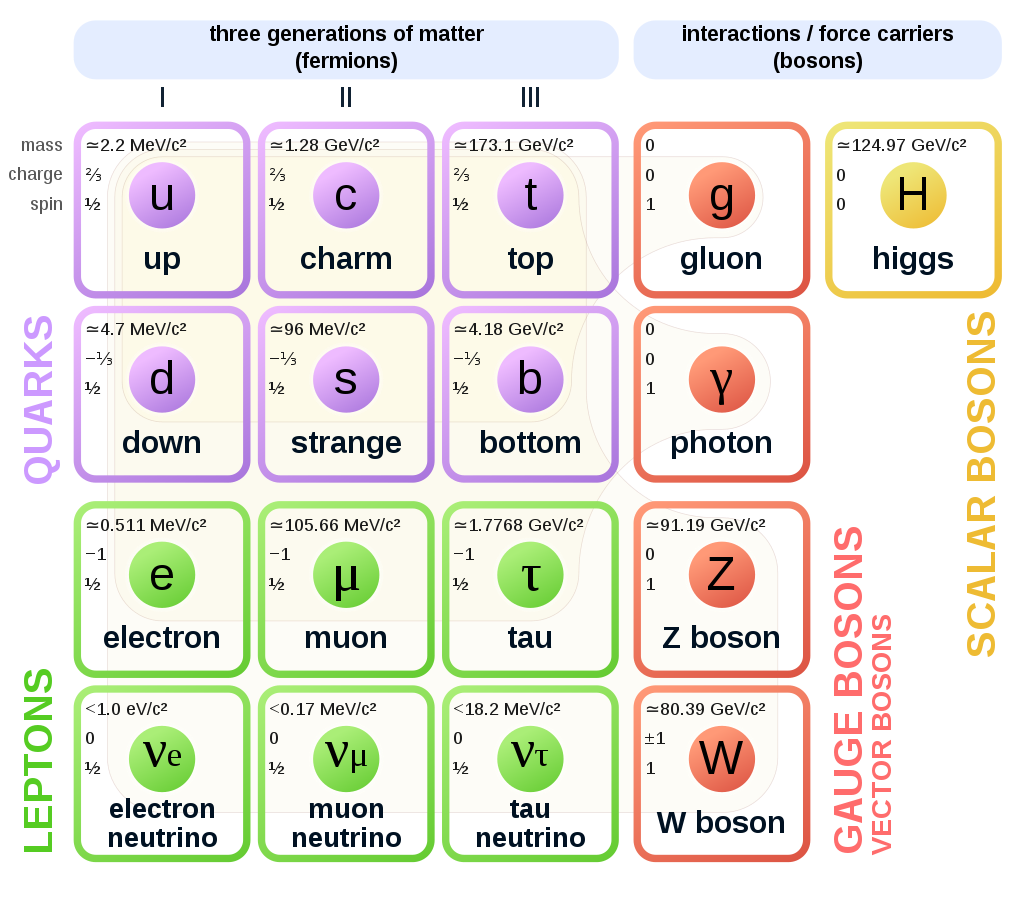
\includegraphics[origin=c,width=0.5\textwidth]{diagrams/3-theory/sm.png}
    \caption[The particles of the Standard Model]
    {The particles of the Standard Model, including the quarks, the leptons and the boson. Figure
        taken from Ref.~\cite{wiki2020}.}
    \label{fig:sm}
\end{figure}

The six quarks and six leptons, all spin $1/2$ particles, are named fermions. Further divided into
three generations (or flavours), they make up all the matter content of the universe. The quarks
never exist in a free state and bind together into mesons or baryons, such as pions and protons,
respectively.  Three charged massive particles, the electron, muon and tau and their three
corresponding (initially assumed to be massless) neutrinos, make up the leptons.

The spin 1 gauge bosons carry the electromagnetic, strong and weak forces. The photon carries the
electromagnetic force (affecting all charged particles), the gluons carry the strong force (which
binds the quarks together), and the massive $Z^{0}$ and $W^{\pm}$ carry the weak force. The final
particle, the Higgs, is a massive scalar boson. Via the process of spontaneous symmetry breaking
it provides the mechanism to give all the particles their mass.

Within the Standard Model neutrinos only interact via the weak force, exclusively coupling to the
$Z^{0}$ and $W^{\pm}$ bosons. As the weak interaction maximally violates parity, in that it only
couples to left-handed chiral particles, the original Standard Model only contains left-handed
neutrinos and their corresponding right-handed anti-neutrinos.

Although neutrinos were initially thought to be massless, and no direct detection of their mass
has been made, it is now believed that neutrinos are massive (albeit very light) particles. This
is due to the substantial amount of evidence in support of neutrino oscillations, some of which
was outlined previously in Section.~\ref{sec:theory_history_osc}. This requires three distinct
neutrino mass states, implying at least two are non-zero.

The Standard Model does not strictly rule out massive neutrinos which may either be \emph{Dirac}
or \emph{Majorana} particles. If neutrinos are Dirac particles, they acquire their mass via a
Yukawa coupling just like the other fermions. This mixes both left-handed and right-handed fields,
requiring the existence of right-handed neutrinos (left-handed antineutrinos) that do not interact
via the weak force. Conversely, if neutrinos are Majorana particles, a mass term is introduced
containing just the left-handed neutrino states. This requires that the neutrino is its own
anti-particle, which as neutrinos do not carry charge, is possible.

Strongly model-dependent cosmological observations of the cosmic microwave background currently
provide the best limit on the combined sum of the neutrino masses at $\sum m_{\nu} <
    0.12~\eV$~\cite{planck2018}. Additionally, the KATRIN experiment has been able to make
model-independent direct measurements of the upper limit by looking at the energy spectrum of
electrons emitted from beta decay, giving a result of $m_{\nu} < 1.1~\eV$~\cite{aker2019}.

\section{Neutrino oscillations} %%%%%%%%%%%%%%%%%%%%%%%%%%%%%%%%%%%%%%%%%%%%%%%%%%%%%%%%%%%%%%%%%%
\label{sec:theory_oscillations} %%%%%%%%%%%%%%%%%%%%%%%%%%%%%%%%%%%%%%%%%%%%%%%%%%%%%%%%%%%%%%%%%%

B. Pontecorvo, Z. Maki, M. Nakagawa, and S. Sakata developed the theory of neutrino oscillations
in the 1960s~\cite{maki1962, pontecorvo1967, pontecorvo1969}. Fundamentally, it is a manifestation
of the phenomenon of quantum interference. If neutrinos are massive, their mass eigenstates are
not necessarily the same as their weakly interacting flavour eigenstates. Instead, the flavour
states are a superposition of the three separate mass states, each propagating as distinct waves
evolving differently with time. As a direct consequence of this, if a neutrino is created with a
specific flavour $\alpha$, its flavour composition will change with time, such that it may later
be detected as having a flavour $\beta$. The probability of this change is found to be periodic
(hence oscillations), and depend on the neutrino energy, the propagation distance, and a
rotational mixing matrix.

\subsection{Neutrino mixing} %%%%%%%%%%%%%%%%%%%%%%%%%%%%%%%%%%%%%%%%%%%%%%%%%%%%%%%%%%%%%%%%%%%%%
\label{sec:theory_oscillations_mixing} %%%%%%%%%%%%%%%%%%%%%%%%%%%%%%%%%%%%%%%%%%%%%%%%%%%%%%%%%%%

The mixing between the flavour eigenstates $\ket{\nu_{\alpha}}$, where $\alpha=e,\mu,\tau$ and the
mass eigenstates $\ket{\nu_{k}}$, $k=1,2,3$, is described by the
\emph{Pontecorvo-Maki-Nakagawa-Sakara} (PMNS) matrix $U$, such that,
\begin{equation} % FLAVOUR AS MASS EQUATION %
    \ket{\nu_{\alpha}}=\sum_{k}^{3}U_{\alpha k}^{*}\ket{\nu_{k}},
\end{equation}
and vice-versa,
\begin{equation} % MASS AS FLAVOUR EQUATION %
    \ket{\nu_{k}}=\sum_{\alpha}^{3}U_{\alpha k}\ket{\nu_{\alpha}}.
\end{equation}
The PMNS matrix is a unitary, complex, $3\times3$ matrix, similar to the Cabibbo-Kobayashi-Maskawa
(CKM) matrix for quark mixing, and has the form,
\begin{gather} % PMNS MATRIX SIMPLE %
    \begin{pmatrix}
        \ket{\nu_{e}}   \\
        \ket{\nu_{\mu}} \\
        \ket{\nu_{\tau}}
    \end{pmatrix}
    =
    \begin{pmatrix}
        U_{e1}     & U_{e2}     & U_{e3}     \\
        U_{\mu 1}  & U_{\mu 2}  & U_{\mu 3}  \\
        U_{\tau 1} & U_{\tau 2} & U_{\tau 3}
    \end{pmatrix}
    \begin{pmatrix}
        \ket{\nu_{1}} \\
        \ket{\nu_{2}} \\
        \ket{\nu_{3}}
    \end{pmatrix}.
\end{gather} %
Three mixing angles and six complex phases can generally describe a $3\times3$ matrix such as
this. However, the majority of these phases can be removed without affecting any physical process.
This leaves three mixing angles $\theta_{12}$, $\theta_{23}$, $\theta_{13}$ and a single phase
$\delta$ which if non-zero produces CP violation and so is commonly named $\delta_{CP}$.

With $s_{ij}=\sin \theta_{ij}$ and $c_{ij}=\cos \theta_{ij}$, the standard parametrisation of
$U$ assuming neutrinos are Dirac particles is given by,
\begin{align} % DIRAC PMNS MATRIX FULL %
    \mathrm{U} & =
    \begin{pmatrix}
        1 & 0       & 0      \\
        0 & c_{23}  & s_{23} \\
        0 & -s_{23} & c_{23}
    \end{pmatrix}
    \begin{pmatrix}
        c_{13}                   & 0 & s_{13}e^{-i\delta_{CP}} \\
        0                        & 1 & 0                       \\
        -s_{13}e^{-i\delta_{CP}} & 0 & c_{13}
    \end{pmatrix}
    \begin{pmatrix}
        c_{12}  & s_{12} & 0 \\
        -s_{12} & c_{12} & 0 \\
        0       & 0      & 1
    \end{pmatrix}
    \label{eq:matrix}
    \\
               & =
    \begin{pmatrix}
        c_{12}c_{13}
         & s_{12}c_{13}
         & s_{13}e^{-i\delta_{CP}}                          \\
        -s_{12}c_{23}-c_{12}s_{23}s_{13}e^{i\delta_{CP}}
         & c_{12}c_{23}-s_{12}s_{23}s_{13}e^{i\delta_{CP}}
         & s_{23}c_{13}                                     \\
        s_{12}s_{23}-c_{12}c_{23}s_{13}e^{i\delta_{CP}}
         & -c_{12}s_{23}-s_{12}c_{23}s_{13}e^{i\delta_{CP}}
         & c_{23}c_{13}
    \end{pmatrix}.
\end{align} %

If neutrinos are instead Majorana in nature two additional phases $\alpha_{21}$ and $\alpha_{31}$
are required, such that the mixing matrix needs to be multiplied by,
\begin{align} % MAJORANA DIAGONAL PMNS EQUATION %
    \mathrm{diag}(1, e^{\frac{i\alpha_{21}}{2}}, e^{\frac{i\alpha_{31}}{2}}).
\end{align} %
Note that both these phases lie on the diagonal and hence have no effect on the oscillations.

\subsection{Oscillations in vacuum} %%%%%%%%%%%%%%%%%%%%%%%%%%%%%%%%%%%%%%%%%%%%%%%%%%%%%%%%%%%%%%
\label{sec:theory_oscillations_vacuum} %%%%%%%%%%%%%%%%%%%%%%%%%%%%%%%%%%%%%%%%%%%%%%%%%%%%%%%%%%%

As the neutrino mass states are eigenstates of the hamiltonian with energy eigenvalues $E_{k}$:
\begin{equation} % HAMILTONIAN EQUATION %
    H \ket{\nu_{k}} = E_{k} \ket{\nu_{k}},
    \label{eq:hamiltonian}
\end{equation}
their time evolution is described by the Schr$\mathrm{\ddot{o}}$dinger equation. This can be used
to determine how the neutrino flavour state, evolves with time, such that,
\begin{equation} % TIME EVOLUTION EQUATION %
    \ket{\nu_{\alpha}(t)}=\sum_{k}^{3}U_{\alpha k}^{*}e^{-iE_{k}t}\ket{\nu_{k}}.
    \label{eq:time_evolution_1}
\end{equation}

After a time $t$, the probability of finding $\ket{\nu_{\alpha}}$ in the state $\ket{\nu_{\beta}}$
is then given by,
\begin{equation} % TIME EVOLUTION EQUATION %
    P(\nu_{\alpha} \rightarrow \nu_{\beta}, t) = |\braket{\nu_{\beta}|\nu_{\alpha}(t)}|^{2}=
    \abs*{\sum_{k}^{3}U_{\alpha k}^{*}U_{\beta k}e^{-iE_{k}t}}^{2} \\
    =\sum_{k}^{3}\sum_{j}^{3}U_{\alpha k}^{*}U_{\beta k}U_{\alpha j}U_{\beta j}^{*}
    e^{i(E_{k}-E_{j})t}.
    \label{eq:osc_prob_1}
\end{equation}
As neutrinos are ultrarelativistic ($p\simeq E$) the approximation can be made that,
\begin{equation} % ENERGY, MASS, MOMENTUM EQUATION %
    E_{k}=\sqrt{\vec{p}_{k}^{\,2}+m_{k}^{2}}\simeq E+\frac{m_{k}^{2}}{2E},
    \label{eq:energy_mass_momentum}
\end{equation}
where $\vec{p}_{k}$ and $m_{k}$ are the neutrino momentum and energy, and $E$ is the neutrino
energy without the mass. This allows the substitution,
\begin{equation} % SUB EQUATION %
    E_{k}-E_{j}\approx\frac{\Delta m_{kj}^{2}}{2E},
    \label{eq:sub}
\end{equation}
where $\Delta m_{kj}^{2}$ is the squared mass difference (\emph{mass splitting}) between the $k$
and $j$ mass states. Additionally, the relativistic limit allows the simplification $t = L$, where
$L$ is the distance from neutrino creation to detection. Combined, the oscillation probability can
be written as,
\begin{align} % TIME EVOLUTION EQUATION %
    P(\nu_{\alpha} \rightarrow \nu_{\beta}, t) = \delta_{\alpha\beta} & - 4\sum_{k>j}re(
    U_{\alpha k}^{*}U_{\beta k}U_{\alpha j}U_{\beta j}^{*})\sin^{2}\left(\frac{\Delta
        m_{kj}^{2}L}{4E}\right) \nonumber
    \\  & \pm 2\sum_{k>j}im(
    U_{\alpha k}^{*}U_{\beta k}U_{\alpha j}U_{\beta j}^{*})\sin\left(\frac{\Delta
        m_{kj}^{2}L}{4E}\right),
    \label{eq:osc_prob_2}
\end{align}
where the last term has a positive sign for neutrinos and a negative sign for anti-neutrinos.

From inspecting Eq.~\ref{eq:osc_prob_2}, the superposition of mass eigenstates is seen to drive
the oscillation of the flavour state, with the amplitude of the oscillation arising from the
elements of the PMNS matrix. Additionally, as a fixed experimental location and neutrino source
define a constant $L/E$, the period of oscillations is determined by the squared mass difference
between the flavour states $\Delta m_{kj}^{2}$.

\subsection{Oscillations in matter} %%%%%%%%%%%%%%%%%%%%%%%%%%%%%%%%%%%%%%%%%%%%%%%%%%%%%%%%%%%%%%
\label{sec:theory_oscillations_matter} %%%%%%%%%%%%%%%%%%%%%%%%%%%%%%%%%%%%%%%%%%%%%%%%%%%%%%%%%%%

As neutrinos propagate through matter, they undergo coherent forward scattering with nucleons.
These interactions do not change the neutrino state or momentum, but they do impart an interaction
potential onto the neutrinos. Two types of interaction can take place, either through the exchange
of a $Z^{0}$ in a \emph{neutral-current} (NC) interaction, or a $W^{\pm}$ in a
\emph{charged-current} (CC) process. The two interaction potentials are given by,
\begin{align} % EFFECTIVE POTENTIAL EQUATION %
    V_{NC} & = \pm\frac{1}{\sqrt{2}}G_{F}n_{n} \\
    V_{CC} & = \pm\sqrt{2}G_{F}n_{e},
\end{align}
were $n_{n}$ and $n_{e}$ are the number density of neutrons and electrons in the medium
respectively and $G_{F}$ is Fermi's constant. The sign of the potential is positive for neutrinos
and negative for anti-neutrinos.

Crucially, as matter is full of electrons but empty of muons or taus, only electron neutrinos can
interact via the CC channel as shown in Fig.~\ref{fig:coherent_scattering}. As a consequence, only
electron neutrinos are affected by the $V_{CC}$ potential, while all flavours are affected by the
$V_{NC}$ potential. When quantitatively applied as an additional potential to the vacuum
hamiltonian, a resonance term is introduced which significantly modifies the vacuum oscillation
probabilities. This effect is know as the Mikheev, Smirnov and Wolfenstein (MSW)
effect~\cite{wolfenstein1978, mikheev1986}.

It is important to note two things. Firstly, a difference between neutrinos and anti-neutrinos is
introduced by the $\pm$ in the $V_{CC}$ potential. Secondly, the modified oscillation probability
is found to be non-symmetric with respect to the sign of the $\Delta m^{2}$ parameters.

\begin{figure} % NUEL COHERENT SCATTERING DIAGRAM %
    \feynmandiagram[vertical'=a to b] {
    i1 [particle=\(\nu_{e}\)]-- [fermion] a-- [fermion] f1 [particle=\(e^{-}\)],
    a -- [boson,edge label=\(W^{\pm}\)] b,
    i2 [particle=\(e^{-}\)]-- [fermion] b-- [fermion] f2 [particle=\(\nu_{e}\)],
    };
    \caption[$\nu_{e}$ coherent scattering Feynman diagram]
    {Feynman diagram of a charged-current coherent scattering interaction between a $\nu_{e}$ and
        an electron.}
    \label{fig:coherent_scattering}
\end{figure}

\section{Neutrino interactions} %%%%%%%%%%%%%%%%%%%%%%%%%%%%%%%%%%%%%%%%%%%%%%%%%%%%%%%%%%%%%%%%%%
\label{sec:theory_interactions} %%%%%%%%%%%%%%%%%%%%%%%%%%%%%%%%%%%%%%%%%%%%%%%%%%%%%%%%%%%%%%%%%%

As outlined in the previous section, there are two types of weak neutrino interactions with
nucleons. Charged-current (CC) and neutral-current (NC) occurring via the exchange of a $Z^{0}$ or
a $W^{\pm}$ respectively. During a CC interaction, the neutrino is transformed into a charged
lepton of the same flavour, conserving charge, flavour, and lepton number as shown in
Fig.~\ref{fig:cc_interaction}. Contrastingly, during an NC interaction, there is no charge or
flavour exchange, and the neutrino continues into the final state as shown in
Fig.~\ref{fig:nc_interaction}.

\begin{figure} % CC DIAGRAM %
    \feynmandiagram[vertical'=a to b] {
    i1 [particle=\(\nu_{l}\)]-- [fermion] a-- [fermion] f1 [particle=\(l^{-}\)],
    a -- [boson,edge label=\(W^{\pm}\)] b,
    i2 [particle=\(n\)]-- [fermion] b-- [fermion] f2 [particle=\(P\)],
    };
    \caption[Feynman diagram of a charged-current interaction.]
    {Example Feynman diagram of a quasi-elastic charged-current interaction of a $\nu_{l}$ with a
        neutron. By identifying the flavour of the charged lepton the flavour of the original
        neutrino can be determined.}
    \label{fig:cc_interaction}
\end{figure}

\begin{figure} % NC DIAGRAM %
    \feynmandiagram[vertical'=a to b] {
    i1 [particle=\(\nu_{l}\)]-- [fermion] a-- [fermion] f1 [particle=\(\nu_{l}\)],
    a -- [boson,edge label=\(Z^{0}\)] b,
    i2 [particle=\(N\)]-- [fermion] b-- [fermion] f2 [particle=\(N\)],
    };
    \caption[Feynman diagram of a neutral-current interaction.]
    {Example Feynman diagram of a neutral-current interaction of a $\nu_{l}$ with a nucleon. The
        flavour of the neutrino can not be identified as there is no charged lepton in the final
        state.}
    \label{fig:nc_interaction}
\end{figure}

CC interactions provide the signal events for the majority of neutrino experiments as the original
neutrino flavour can be determined via identification of the charged lepton. Conversely, NC
interactions are background events as there is no way to identify the original neutrino without a
charged lepton and when the cross-sections are constant across all neutrino flavours in the NC
case.

For \chips the relevant neutrino interaction energy regime is commonly referred to as the
\emph{transition region}, covering a range of energies between 1 and \unit{10}{\GeV}. Both CC and
NC interactions within this regime fall into one of five main categories outlined below.

\begin{itemize}
    \item \textbf{Quasi-Elastic(elastic) Scattering (QE)} is the dominant channel for energies
          below \unit{1}{\GeV} and involves the neutrino scattering off the entire nucleon. In the
          CC neutrino case, this converts the target neutron to a proton which is reversed for
          anti-neutrinos. The same process can also occur in an NC interaction, where it is often
          referred to as \emph{elastic} scattering.

    \item \textbf{Meson Exchange Current (MEC)} provides an additional contribution to the energy
          range dominated by QE interactions. The interaction involves two nucleons and produces
          two protons in the final state. Sometimes referred to as the \emph{2p2h} interaction it
          has become essential for explaining the discrepancy between theory and observations
          within many modern experiments and is now included by default in popular event
          generators~\cite{katori2013}.

    \item \textbf{Resonant Pion Production (Res)} is the dominant channel between 1 and
          \unit{2}{\GeV} and involves the neutrino exciting the target nucleon into a resonant
          state. The resonance then decays the vast majority of the time to produce a single pion
          and nucleon in the final state. This can happen via three CC channels and four NC
          channels. This production mechanism is responsible for the majority of NC single
          $\pi^{0}$ events within water Cherenkov detectors such as \chips. This channel,
          discussed further in Section.~\ref{sec:chips_cherenkov}, forms an incredibly difficult
          component of the background to deal with as it can mimic electrons.

    \item \textbf{Coherent Pion production (Coh)} is a much rarer interaction mechanism where the
          neutrino scatters coherently from the entire nucleus. This process transfers negligible
          energy to the target and produces a significantly forward scattered pion with no nuclear
          recoil in the final state.

    \item \textbf{Deep inelastic scattering (DIS)} is dominant for neutrino energies above
          \unit{3}{\GeV} with the additional energy allowing for the neutrino to resolve the
          individual quark content of the nucleon. The subsequent scattering off an individual
          quark produces a hadronic shower in the final state, containing multiple pions which are
          often a challenge to reconstruct.
\end{itemize}

The standard $\nu_{e}$ (very similar to $\nu_{\mu}$) cross-sections included with the GENIE event
generator~\cite{andreopoulos2009, andreopoulos2015} for all the above processes are shown in
Fig.~\ref{fig:xsec_nu_e_O16} for both CC and NC interactions. For $\nu_{\tau}$ interactions the CC
cross-sections differ considerably due to the large $\tau$ lepton mass as shown in
Fig.~\ref{fig:tau_comparison} only becoming non-negligible for energies above
$\approx\unit{5}{\GeV}$.

\begin{figure} % XSEC NUEL DIAGRAM %
    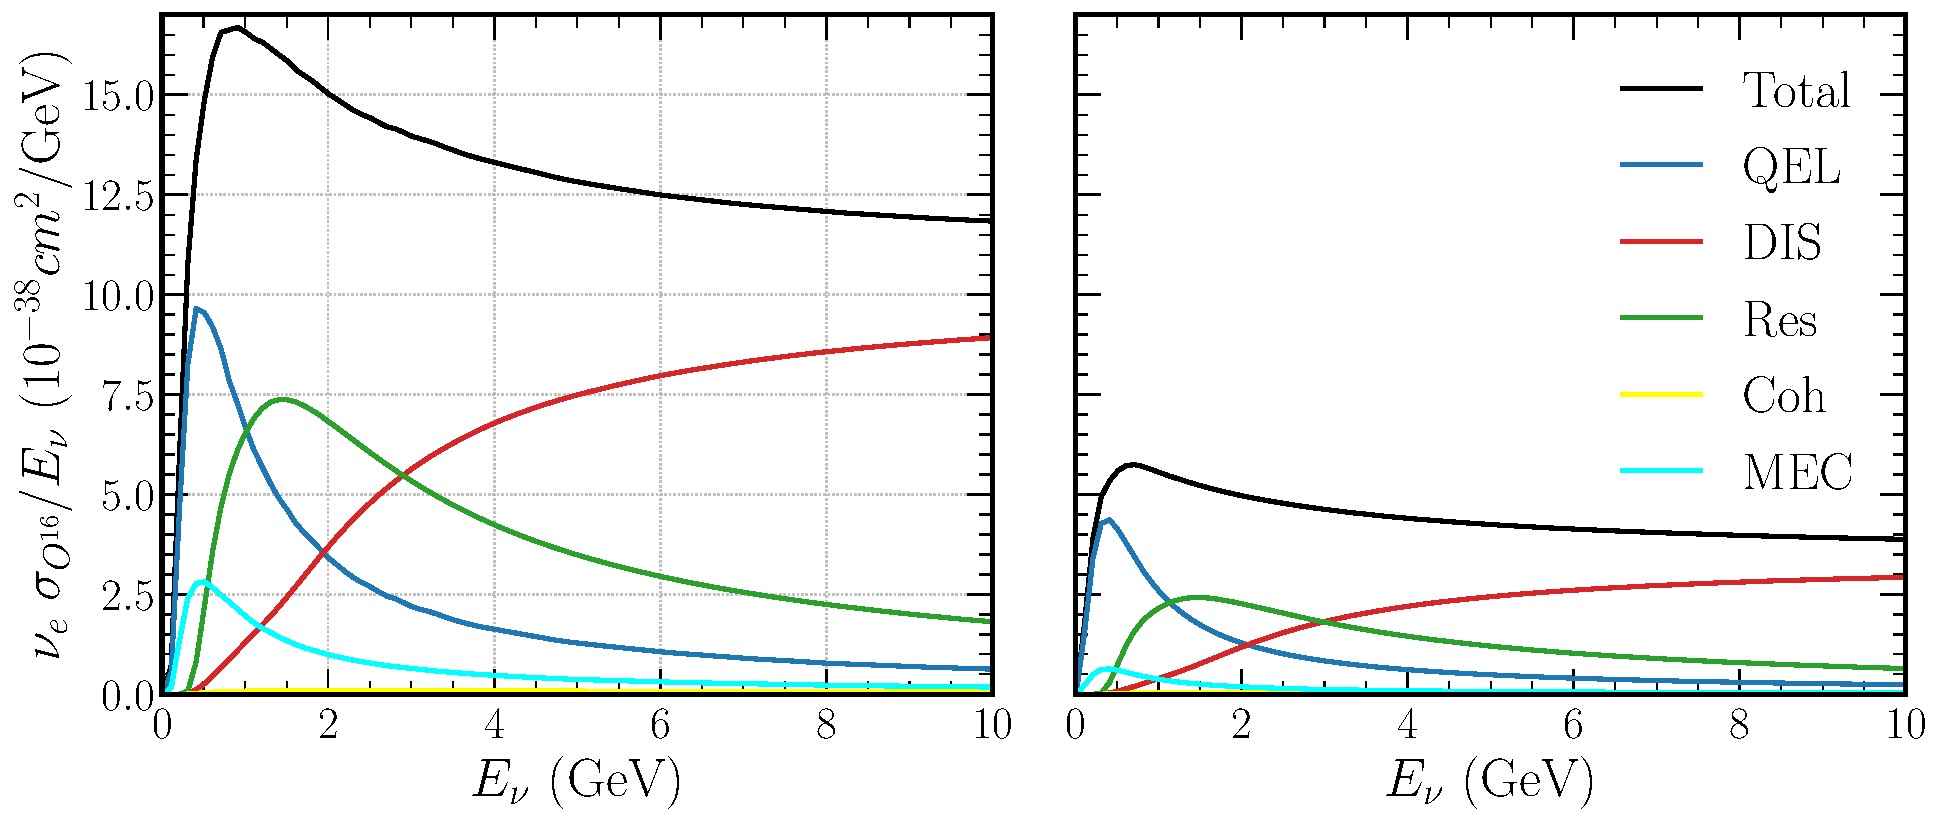
\includegraphics[width=\textwidth]{diagrams/3-theory/xsec_nu_e_O16.pdf}
    \caption[$\nu_{e}$ GENIE cross-sections on Oxygen-16.]
    {Example GENIE cross-sections for CC $\nu_{e}$ (left) and NC $\nu_{e}$ (right). Shown are the
        total and contributing process cross-sections on Oxygen-16. Note how the total
        cross-section approaches a linear dependence on energy and the NC cross-sections are
        smaller than their CC counterparts.}
    \label{fig:xsec_nu_e_O16}
\end{figure}

\begin{figure} % TAU CROSS-SECTION DIAGRAM %
    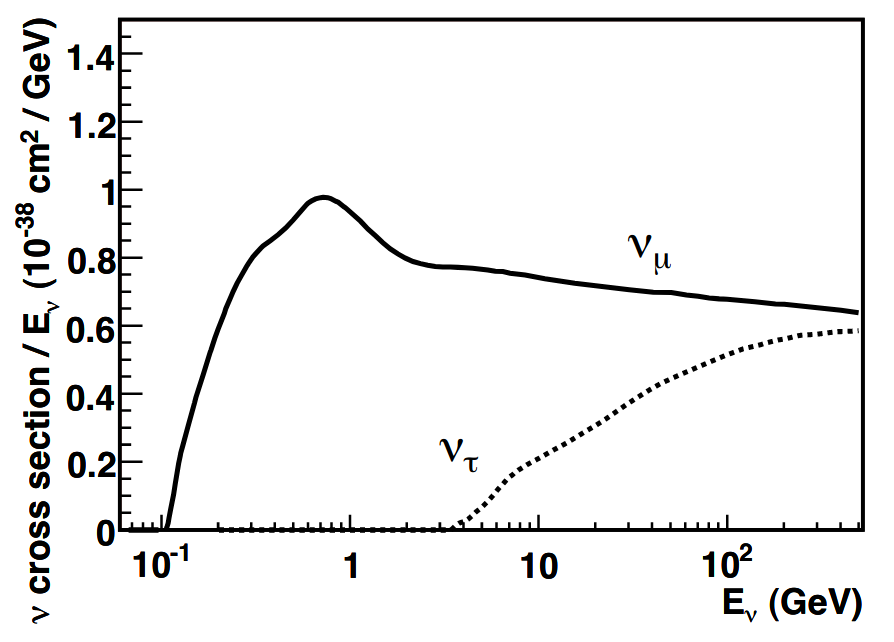
\includegraphics[origin=c,width=0.5\textwidth]{diagrams/3-theory/tau_comparison.png}
    \caption[tau comparison short]
    {Comparison of the total CC interaction cross-sections per nucleon divided by the neutrino
        energy for $\nu_{\mu}$ and $\nu_{\tau}$. Figure taken from Ref.\cite{formaggio2012}.}
    \label{fig:tau_comparison}
\end{figure}

\section{Current status and the future}

The three-component representation of the PMNS matrix presented in Eq.~\ref{eq:matrix} splits our
understanding of neutrino oscillations into three sectors. Historically, this separated
experiments observing different sources of neutrinos, from either the sun, atmosphere or nuclear
reactors. Hence the standard names given to each: the \emph{solar sector}, \emph{atmospheric
    sector}, and \emph{reactor sector}. However, it is perhaps more rigorous to think of each sector
as corresponding to the PMNS parameters they encompass: $\Delta m^{2}_{21}$ and $\theta_{12}$ for
the solar sector, $\Delta m^{2}_{32}$ and $\theta_{23}$ for the atmospheric sector, and
$\theta_{13}$ for the reactor sector.

During the last couple of decades the focus of experiments in each of these sectors has shifted
from the discovery of neutrino fundamentals to precision measurement. This is led to a
corresponding shift in using increasingly abundant neutrino sources and larger and larger
detectors. Below we outline the current status, open questions, and what the future holds for
neutrino physics.

\subsection{Current status} %%%%%%%%%%%%%%%%%%%%%%%%%%%%%%%%%%%%%%%%%%%%%%%%%%%%%%%%%%%%%%%%%%%%%%
\label{sec:theory_status_current} %%%%%%%%%%%%%%%%%%%%%%%%%%%%%%%%%%%%%%%%%%%%%%%%%%%%%%%%%%%%%%%%

Global fits to neutrino oscillation data aggregate the most up-to-date results from multiple
experimental sources, some of which are outlined below, to constrain the parameters of the PMNS
matrix. The latest best fit results from one such global fit,
NuFIT~\cite{esteban2019,esteban2020}, are shown in Fig.~\ref{fig:best_fit}.

\begin{figure} % BEST FIT DIAGRAM %
    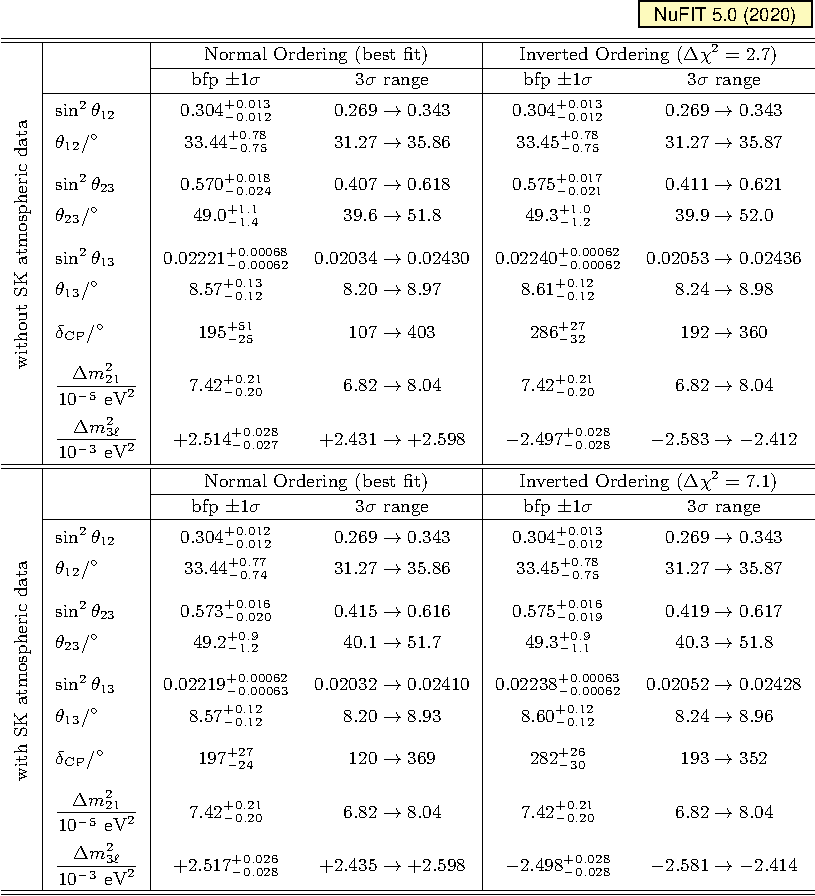
\includegraphics[origin=c,width=0.8\textwidth]{diagrams/3-theory/best_fit.pdf}
    \caption[best fit short]
    {Three-flavour results from the NuFIT v5.0 global fit as of July 2020, showing both 1$\sigma$
        uncertainties and $\pm 3 \sigma$ ranges. The first column shows the results for the normal
        hierarchy and the second for the inverted hierarchy. Additionally, the lower section
        includes atmospheric neutrino data from the Super-Kamiokande experiment, while the upper
        section does not. Figure taken from Ref.~\cite{esteban2020}.}
    \label{fig:best_fit}
\end{figure}

\subsubsection*{Solar parameters: $\theta_{12}$ and $\Delta m^{2}_{21}$} %%%%%%%%%%%%%%%%%%%%%%%%%

- Homestake chlorine~\cite{cleveland1998}
- SNO combined results~\cite{maneira2011} mentioned earlier
- GALLEX updated results~\cite{kaether2010} mentioned earlier gallium
- SAGE latest results~\cite{abdurashitov2009} mentoned earlier gallium
- Super-Kamiokande, water Cherenkov detector, 1km underground, 40m diameter, 40m tall, 50kt of
pure water. Observed by 11 thousand 20 inch MTs detecting Cherenkov light.
- super-kamiokande 1 solar results~\cite{hosaka2006}
- super-kamiokande 2 solar results~\cite{cravens2008}
- super-kamiokande 3 solar results~\cite{abe2011_super}
- super-kamiokande combined solar results~\cite{nakano2017}
- Borexino 1~\cite{bellini2011} -  liquid scintillator experiment
- Borexino 2~\cite{Bellini2010}
- Borexino 3~\cite{bellini2014}
- KamLAND solar~\cite{gando2011} - Liquid Scintillator Antineutrino Detector underground

- The rightmost sub-matrix of REF describes the solar sector
- Experiments detector neutrinos created in the sun are sensitive to
- The mixing angle $\theta_{12}$ and the mass difference $\Delta m^{2}_{21}$
- Initially from experiments looking at solar neutrino problem mentioned above
- Homestake then solved by SNO etc...
- Heavily dominated by MSW effect, because of high sun electron density, leading to large
resonance increasing nuel to numu transitions.
- In addition to experiments mentioned earlier KamLAND has probed this sector to confirm the
parameters.
- Dominant results in this sector are due to SNO and KamLAND experiments.
- Combined SNO fits collector from its three run configurations.
- KamLAND was a reactor neutrino experiment consisting of a 1 kton liquid scintillator detector
- Positioned between several nuclear reactors

\subsubsection*{Atmospheric parameters: $\theta_{23}$ and $\Delta m^{2}_{32}$} %%%%%%%%%%%%%%%%%%%

- Conventional super-k~\cite{abe2018}
- Conventional IceCube DeepCore~\cite{aartsen2015}
- Amundsen–Scott South Pole Station in Antarctica. Uses PMTs arranged in DOMs under the ice
- Accelerator/beam experiments. Nova, Fermilab minnesota.
- MINOS atm~\cite{adamson2013_1,adamson2013_2}
- NoVA atm~\cite{acero2019,himmel2020}
- Uses same SUper-K but a beam of neutrinos as well for JParc
- T2k atm~\cite{dunne2020}

- The leftmost sub-matrix of REF describes the atmospheric sector
- Experiments looking at neutrinos produced in cosmic ray interactions in the upper atmosphere
- The mixing angle $\theta_{23}$ and the mass difference $\Delta m^{2}_{32}$
($\approx\Delta m^{2}_{31}$)
- Accelerator experiments looking at $P(\nu_{\mu}\rightarrow\nu_{\mu})$.
- Kamiokande and IMB background mentioned earlier.
- A deficit just like in solar sector \emph{atmospheric neutrino anomaly}.
- Probed using atmospheric neutrinos and accelerator neutrinos.
- Primarily muon neutrinos can be produced by using a particle accelerator to direct a proton beam
at a target. By focusing the pions and kaons this produces, a neutrino beam created from the
downstream decays, creates the muon neutrino beam.
- Main channel relevant to this sector in muon neutrino survival.

\subsubsection*{Reactor parameter: $\theta_{13}$} %%%%%%%%%%%%%%%%%%%%%%%%%%%%%%%%%%%%%%%%%%%%%%%%

- KamLAND theta13~\cite{eguchi2002,gando2013}
- Daya bay theta13~\cite{an2012,an2017}
- RENO theta13~\cite{ahn2012,bak2018}
- Double Chooz theta13~\cite{abe2012}
Accelerator experiments have also found not as good but consistent values
- Minos appearance~\cite{adamson2013_3}
- T2K appearance~\cite{abe2013}
- NoVA appearance~\cite{adamson2016_2}

- Reactor experiments have become sensitive enough to measure the survival probability for
electron antineutrinos $P(\bar{\nu_{e}}\rightarrow\bar{\nu_{e}})$.
- With the measurements of a non-zero theta13 by reactor neutrino experiments, the main focus now
has shifted to resolving the mass hierarchy ambiguity and measuring delta-cp. These can be probed
by long-baseline neutrino experiments by looking to numu to nuel transitions.

\subsection{Open Questions} %%%%%%%%%%%%%%%%%%%%%%%%%%%%%%%%%%%%%%%%%%%%%%%%%%%%%%%%%%%%%%%%%%%%%%
\label{sec:theory_status_open} %%%%%%%%%%%%%%%%%%%%%%%%%%%%%%%%%%%%%%%%%%%%%%%%%%%%%%%%%%%%%%%%%%%

There are still many open questions regarding the various parameters of the PMNS matrix. After
briefly outlining them below, discussion of how current and future experimental efforts aim to
resolve these questions will be outlined in the following chapter.

\subsubsection*{Octant of $\theta_{23}$} %%%%%%%%%%%%%%%%%%%%%%%%%%%%%%%%%%%%%%%%%%%%%%%%%%%%%%%%%

It is known that the mixing angle $\theta_{23}$ is non-zero and large. Initially thought to be
maximal such that, $\theta_{23}=\pi/4=45^{\circ}$, we now know that this is not the case. However,
it is still unclear if $\theta_{23}<45^{\circ}$ or $\theta_{23}>45^{\circ}$, commonly referred to
as the octant. Although easily measured be studying $\nu_{\mu}$ disappearance, a degeneracy in the
oscillation probability removes the ability to determine the octant. $\nu_{e}$ appearance,
however, contains an oscillation term allowing for the octant to be resolved, but an exploration
of this channel is yet to produce a significant result.

\subsubsection*{Mass hierarchy} %%%%%%%%%%%%%%%%%%%%%%%%%%%%%%%%%%%%%%%%%%%%%%%%%%%%%%%%%%%%%%%%%%

Neutrino oscillation experiments allow us to measure the mass squared differences between the
neutrino mass states. The value of $\Delta m_{21}^2$ has been measured by solar neutrino
experiments and is known to be small and positive. Meaning that $m_{2}>m_{1}$ where $m_{1}$ is
defined to be the dominant mass state of the electron neutrino. However, the sign of $\Delta
    m_{32}^2$ is currently unknown. This allows for two possible scenarios, either $m_1<m_2<m_3$,
known as normal hierarchy, or $m_3<m_1<m_2$, known as inverted hierarchy. Both are illustrated in
Fig.~\ref{fig:hierarchy}.

Oscillations in vacuum are not sensitive to the sign of the $\Delta m^{2}$ parameters. However,
matter effects allow for the sign to be determined. Resolving this ambiguity will significantly
improve the ability of experiments to both determine the value of $\delta_{CP}$ and discover if
neutrinos are Dirac or Majorana in nature.

- Best bet is long-baseline accelerator experiments as their neutrinos have travelled a long
distance through material for it to take effect.
- JUNO medium baseline reactor experiment will solve this~\cite{an2016}

\begin{figure} % MASS HIERARCHY DIAGRAM %
    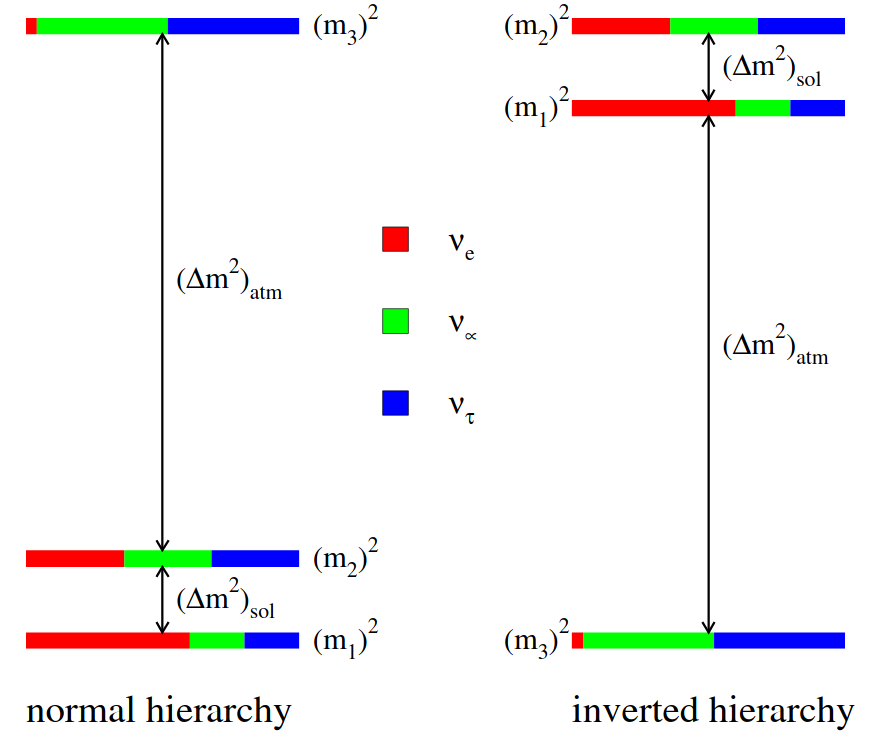
\includegraphics[origin=c,width=0.5\textwidth]{diagrams/3-theory/hierarchy.png}
    \caption[Illustration of the two possible mass hierarchies]
    {Illustrated diagram of the two possible mass hierarchies. The atmospheric (atm) and solar
        (sol) naming convention is used for the mass differences. The sign of
        $\Delta m_{21}^{2}$ is small and positive, while the sign of $\Delta m_{32}^{2}$ is
        unknown. Figure taken from Ref.~\cite{gouvea2013}.}
    \label{fig:hierarchy}
\end{figure}

\subsubsection*{CP-violation} %%%%%%%%%%%%%%%%%%%%%%%%%%%%%%%%%%%%%%%%%%%%%%%%%%%%%%%%%%%%%%%%%%%%

The current level of CP violation observed in the quark sector does not fully explain the
matter-antimatter asymmetry of the universe. However, if CP violation is shown to exist in the
leptonic sector, leptogenesis models of the early universe allow this to go some way to resolving
the issue. The PMNS matrix allows for $P(\nu_{\alpha}\rightarrow\nu_{\beta}) \neq
    P(\bar{\nu_{\alpha}}\rightarrow\bar{\nu_{\beta}})$, when $\delta_{CP}$ is not 0 or $\pi$. The most
promising channel for this measurement is $\nu_{e}$ appearance from a $\nu_{\mu}$ neutrino source,
where the oscillation probabilities change significantly, as shown in Fig.~\ref{fig:osc_cp_probs}.

\begin{figure} % OSCILLATION CP PROBS DIAGRAM %
    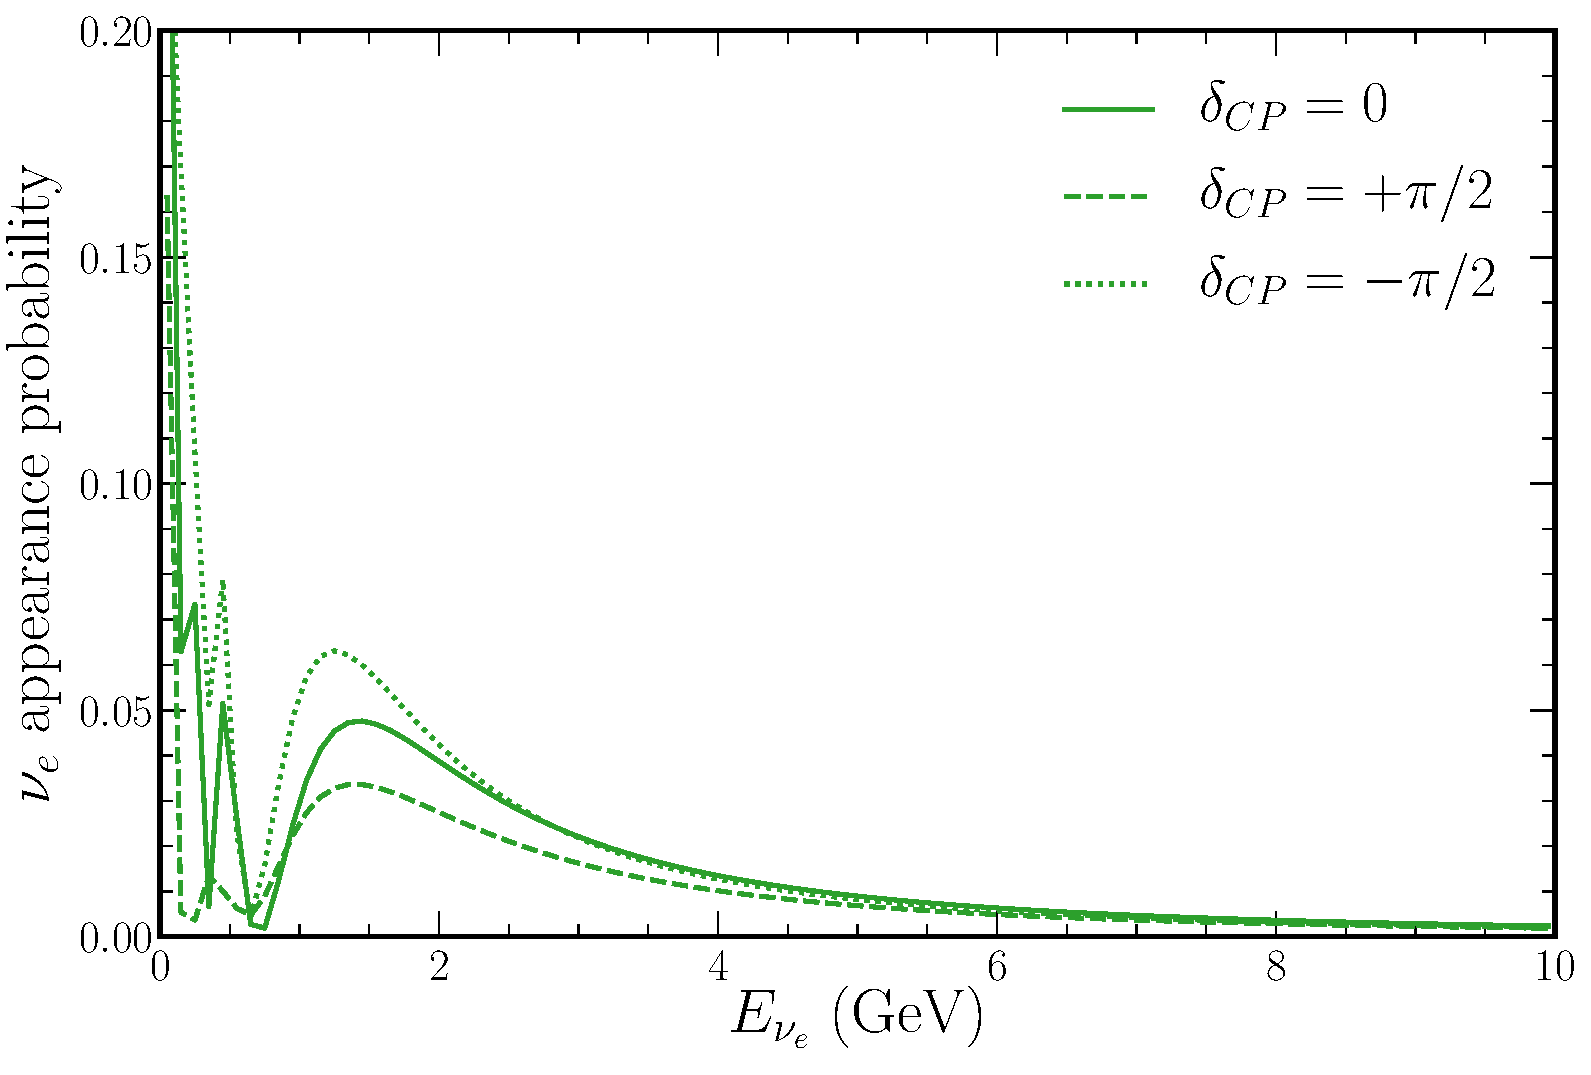
\includegraphics[origin=c,width=0.7\textwidth]{diagrams/6-cvn/chipsnet/explore_osc_cp_probs.pdf}
    \caption[$\nu_{e}$ appearance probability for different $\delta_{CP}$ values]
    {Appearance probability of $\nu_{e}$ oscillating from $\nu_{\mu}$ at $L=712$ km. The
        oscillations are show for three different values of $\delta_{CP}$.}
    \label{fig:osc_cp_probs}
\end{figure}

- Provide tantalising hints at a non zero value
- NoVA delta-cp~\cite{acero2019}
- T2k delta-cp~\cite{abe2018_2}

\subsection{The future} %%%%%%%%%%%%%%%%%%%%%%%%%%%%%%%%%%%%%%%%%%%%%%%%%%%%%%%%%%%%%%%%%%%%%%%%%%
\label{sec:theory_status_future} %%%%%%%%%%%%%%%%%%%%%%%%%%%%%%%%%%%%%%%%%%%%%%%%%%%%%%%%%%%%%%%%%

Hyper-k letter of intent~\cite{abe2011}
Dune CDR~\cite{acciarri2016}

Two large-scale long-baseline experiments are under preparation or proposed in future. DUNE
    [103]will be a 1,300 km long-baseline experiment based in US. The DUNE far detector will consist
offour modules of at least 10 kt fiducial mass liquid argon time projection chambers, located 1.5
kmunderground at the Sanford Underground Research Facility in South Dakota. The beamline forDUNE,
1.2 MW at start and upgradable to 2.4 MW, as well as the facility for near detectors willbe newly
constructed at Fermilab. In Japan, Hyper-Kamiokande [102] is proposed as the succes-sor of the
Super-Kamiokande detector. It will be a water Cherenkov detector with 260 (190) kttotal (fiducial)
mass. With upgrade of existing accelerator and beamline, J-PARC will provide a1.3 MW neutrino beam
to Hyper-Kamiokande. Both DUNE and Hyper-Kamiokande will have arich physics program besides the
long-baseline experiment, such as searches for nucleon decays andstudy of supernova neutrinos.

- They can also study atmospheric neutrinos


- BIG EQUATION FOR PROBABILITY: shows sensitivity to the mass hiearchy through the matter effect
parameters A and to the cp-violtating phase trhough the second term.
- Over that last 20 years neutrino oscillations have become well-established and we are now moving
into the precision measurement era.
- DUNE is a next-generation neutrino oscillation experiment with a primary scientific goal of
observation of CP-violation in the neutrino sector.
- In DUNE a muon neutrino(anti-neutrino) beam will be produced by the Long-Baseline Neutrino
Facility (LBNF)
- There will be a near detector at Fermilab before the neutrinos travel the 1285km to the Sanford
Underground Research Facility (SURF) in South Dakota.
- The far detector will consist of four 10kt (fiducial) liquid argon time projections chamber
(LArTPC) detectors.
- Neutrino oscillation probabilities can then be infered by comparisons of the observed neutrino
spectra and the near and far detectors.
- Recent obsevation of a large theta13 have focuseed the next genetation of long baseline
experiments towards the mass hierarchy, octant of theta23 and measureing delta-CP
- Nova and T2k will not be able to measure the remaining unknows (check this)
- Dune will hopefully solve these problems but will be increadibly expensive

- Symmetries under charge-conjugation and parity inversion are both macimally violated by the
waek interaction.
- Their combined operation has been shown to be violated, to a small degress, by quark mixing
processes.
- If sin(delta-cp) is non zero then vacuum oscillation properties of nu and anti nu will be
different.
- DUNE (I assume CHIPS) is sensative to four oscillation paramters, delta31, theta23, theta13
and delta-cp.
- These can be measured using four data sample, two for neutrino and two for antineutrinos.
- These sample are produced by "Forward Horn current" FHC and "Reverse Horn current" RHC,
producing predominetetly neutrinos and anti-neutrinos respectively.
- Dissapearence channels sensitive to %abs(delta31^2), and sin^2(2theta23).
- Apperence channels sensitive to all four parameters including sign of %delta32^2.
- The "signal" in all cases are CC interactions, therefore selection of nuel, anuel, numu and
anumu CC is the goal.
- Main background in CC numu selections are NC with charged pions.
- Main background in CC nuel selections is pi-zero NC, which can mimic the chracteristic EM
shower, due to its near certain decay into two photons.
- You get a small number of nuel intrinsic to the beam, they are just a background as they are
indistinguishabe from the nuel appreaence neutrinos.
- Once you have collected samples in all four cases, a fit is performed to the reconstructed
neutrino energy distributions to extract the four neutrino oscillation parameters.